
%\begin{figure}
%	\begin{center}
%		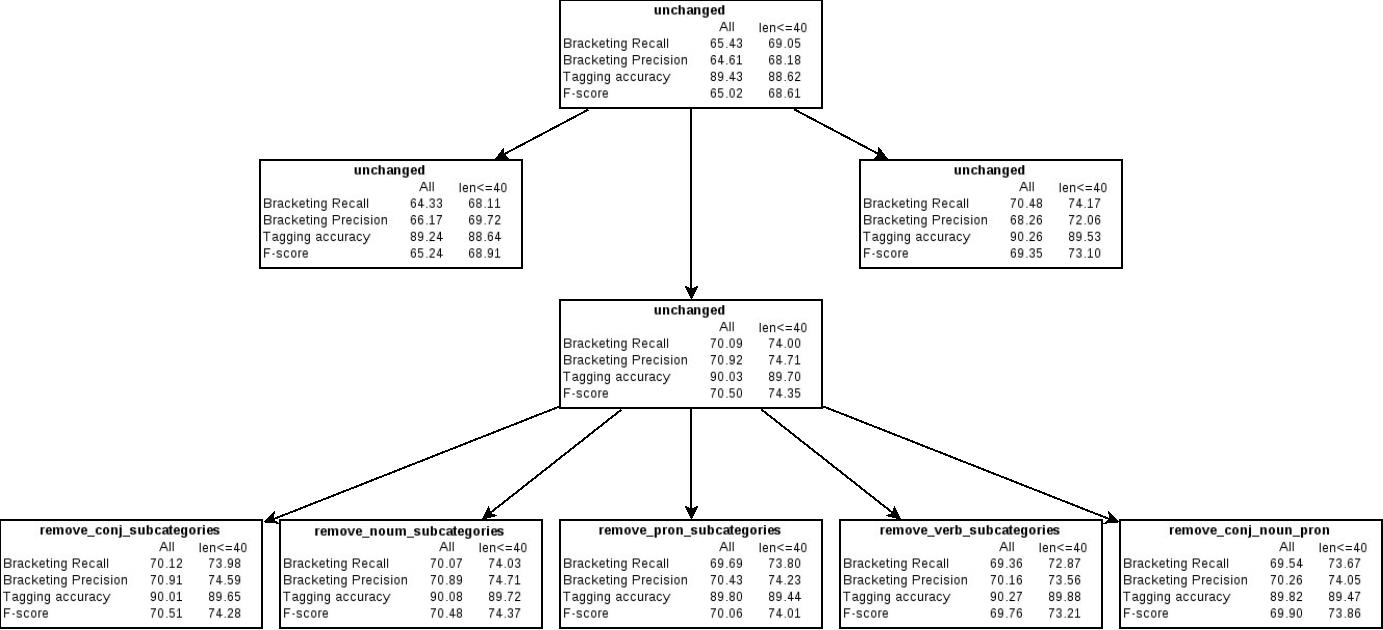
\includegraphics[scale=0.35]{diagrama_experimentos2.jpeg}
%		\caption{\label{evolucao} Evolução dos resultados }		
%	\end{center}
%\end{figure}

Primeiro teste

Regras de \emph{head-find} usadas:

\scriptsize
\begin{verbatim}
  (
  (NP (l N PROP PRON-PERS PRON-INDP N-ADJ NP))
  (VP (l V-FIN V-INF V-PCP V-GER) (l VP))
  (ADJP (l ADJ ADJP) (l PRON-DET))
  (ADVP (r ADV ADVP))
  (CU (r CONJ-C CU , ;))
  (X (l VP))
  (PP (l PRP PP))
  (FCL (l VP) (l NP))
  (ICL (l VP) (l NP))
  (ACL (l VP) (l NP))
  (* (l))
  )
\end{verbatim}

Resultados obtidos

\begin{verbatim}
  Bracketing Recall         =  62.38
  Bracketing Precision      =  68.80
  Tagging accuracy          =  58.84
\end{verbatim}

\normalsize
Achamos que os resultados estavam baixos devido as TAGS de anotação dos verbos possuírem um hífen, e o \emph{parser} não reconhece o hífen como parte da TAG.

Segundo teste

Alteramos as \emph{tags} que possuíam o caractere hífen (``-''), pois o \emph{parser} desconsidera a parte a direita do mesmo, e o programa de avaliação não. Por isso os resultados da avaliação são prejudicados.

As regras de \emph{head-find} foram alteradas para:

\scriptsize
\begin{verbatim}
  (
  (NP (l N PROP PRONPERS PRONINDP NADJ NP))
  (VP (l VFIN VINF VPCP VGER) (l VP))
  (ADJP (l ADJ ADJP) (l PRONDET))
  (ADVP (r ADV ADVP))
  (CU (r CONJC CU , ;))
  (X (l VP))
  (PP (l PRP PP))
  (FCL (l VP) (l NP))
  (ICL (l VP) (l NP))
  (ACL (l VP) (l NP))
  (* (l))
  )
\end{verbatim}

Resultados obtidos

\begin{verbatim}
  Bracketing Recall         =  61.47
  Bracketing Precision      =  68.20
  Tagging accuracy          =  79.83
\end{verbatim}

\normalsize
Apenas a precisão das tags melhorou, porém não houve melhora nas métricas \emph{Bracketing Recall} e \emph{Bracketing Precision}.

Terceiro teste

No próximo teste pretendemos verificar o quanto o \emph{parser} consegue melhorar seu desempenho quando não tem que especificar se o verbo esta em uma das quatro categorias, tendo apenas a anotação genérica de verbo.

As regras de \emph{head-find} foram alteradas para:

\scriptsize
\begin{verbatim}
  (
  (NP (l N PROP PRONPERS PRONINDP NADJ NP))
  (VP (l V) (l VP))
  (ADJP (l ADJ NUM) (l ADJP) (l PRONDET))
  (ADVP (r ADV ADVP))
  (CU (r CONJC CU , ;))
  (X (l VP))
  (PP (l PRP PP))
  (FCL (l VP) (l NP))
  (ICL (l VP) (l NP))
  (ACL (l VP) (l NP))
  (* (l))
  )
\end{verbatim}

Resultados obtidos


\begin{verbatim}
  Bracketing Recall         =  60.42
  Bracketing Precision      =  67.42
  Tagging accuracy          =  80.73
\end{verbatim}

\normalsize
Novamente, a precisão das tags aumentou, porém o \emph{Precision} e \emph{Recall} diminuíram. A generalização da tag V fez com que categorias sintáticas externas como ICL, ACL e FCL fossem influenciadas.

Quarto teste

Como já verificado com as tags, o \emph{parser} também exibe problemas com o caractere hífen (``{-}'') no texto. Após substituir todos os hífens por \emph{underscore} (``\_''), os resultados obtidos foram melhores.

As regras de \emph{head-find} são as mesmas.

\scriptsize
\begin{verbatim}
  (
  (NP (l N PROP PRONPERS PRONINDP NADJ NP))
  (VP (l V) (l VP))
  (ADJP (l ADJ NUM) (l ADJP) (l PRONDET))
  (ADVP (r ADV ADVP))
  (CU (r CONJC CU , ;))
  (X (l VP))
  (PP (l PRP PP))
  (FCL (l VP) (l NP))
  (ICL (l VP) (l NP))
  (ACL (l VP) (l NP))
  (* (l))
  )
\end{verbatim}

Resultados obtidos

\begin{verbatim}
  Bracketing Recall         =  67.42
  Bracketing Precision      =  68.09
  Tagging accuracy          =  90.36
\end{verbatim}

\normalsize

Percebemos uma melhora significativa nos valores de \emph{Bracketing Recall} e \emph{Tagging accuracy}, a partir de agora sempre substituiremos os caracteres ``{-}'' por ``\_''.

Quinto teste

Na próxima experiência vamos utilizar novamente a especialização das categorias de verbo e com um corpus de desenvolvimento e teste maior.

\scriptsize

\begin{verbatim}
  (
  (NP (l N PROP PRONPERS PRONINDP NADJ NP))
  (VP (l VFIN VINF VPCP VGER) (l VP))
  (ADJP (l ADJ ADJP) (l PRONDET))
  (ADVP (r ADV ADVP))
  (CU (r CONJC CU , ;))
  (X (l VP))
  (PP (l PRP PP))
  (FCL (l VP) (l NP))
  (ICL (l VP) (l NP))
  (ACL (l VP) (l NP))
  (* (l))
  )
\end{verbatim}


Resultados obtidos


\begin{verbatim}
  Bracketing Recall         =  72.50
  Bracketing Precision      =  72.73
  Tagging accuracy          =  90.46
\end{verbatim}

\normalsize
Verificamos uma melhora expressiva em relação aos primeiros testes realizados após a retirada dos hífens das \emph{tags} de categoria de verbos e após a substituição dos caracteres ``{-}'' por ``\_''.

Uma avaliação mais aprofundada será feita posteriormente. 
